\section{Activity}

On the figure \ref{fig:activity_by_hour}, the activity of programmers by hour is presented. It is measured in two ways: by counting the data points generated in distinct hours, and by summing the actions within these data points. I remind that \texttt{actions} is an attribute of a data point \ref{sec:data_description} and here I sum these attributes of multiple data points. In both cases of measurement the \texttt{start} timestamp determines the hour bucket where a data point or an action falls under. Timezone from the timestamps is ignored here and in analogous graphs later. Thus, for instance, two programmers working at 10:00 in Warsaw and at 10:00 in San Francisco on the same day would contribute to the same hour bucket. On the graph it is clearly observed in both of the measurement ways that most of the activity happens in the afternoon and that the work almost completely ceases in the middle of the night and around dawn.

\begin{figure}[htbp]
  \centering
  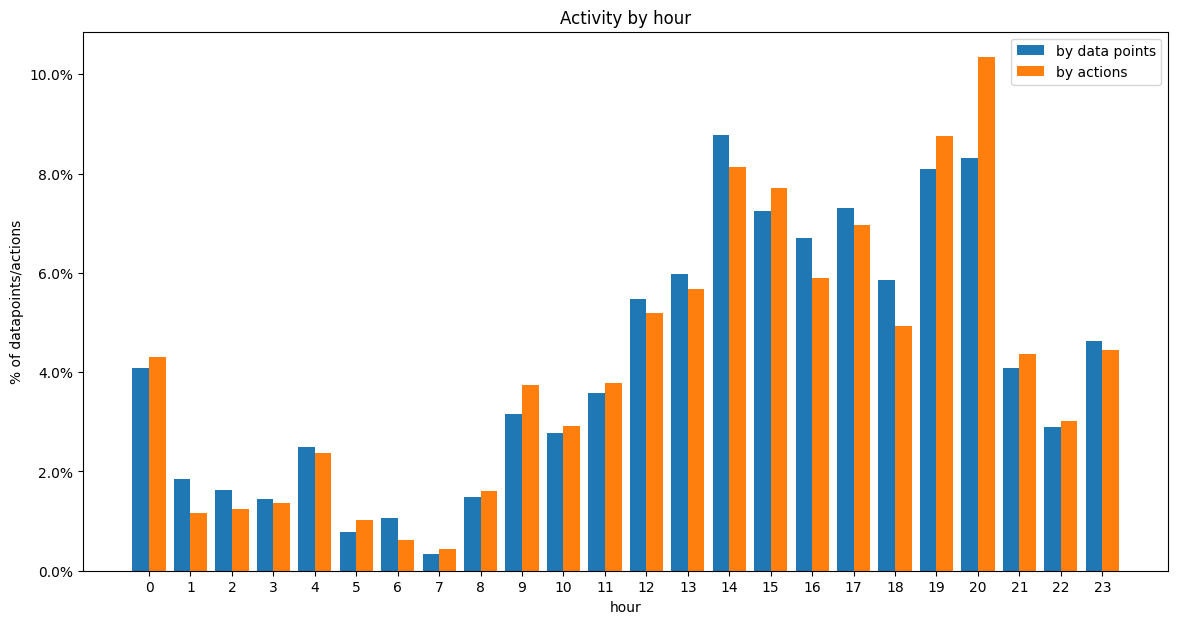
\includegraphics[scale=0.5]{chapters/results/graphics/activity-by-hour.png}
  \caption{Comparison of activity by hour with regards to data points and actions}
  \label{fig:activity_by_hour}
\end{figure}

Similar observations can be made by examining the activity graph with respect to different programming languages \ref{fig:activity_by_hour_langs}. The noticeable difference may be that for JS/TS developers the activity is strongly concentrated in the afternoon where for Python developers some activity is also observed during the night.

\begin{figure}[htbp]
  \centering
  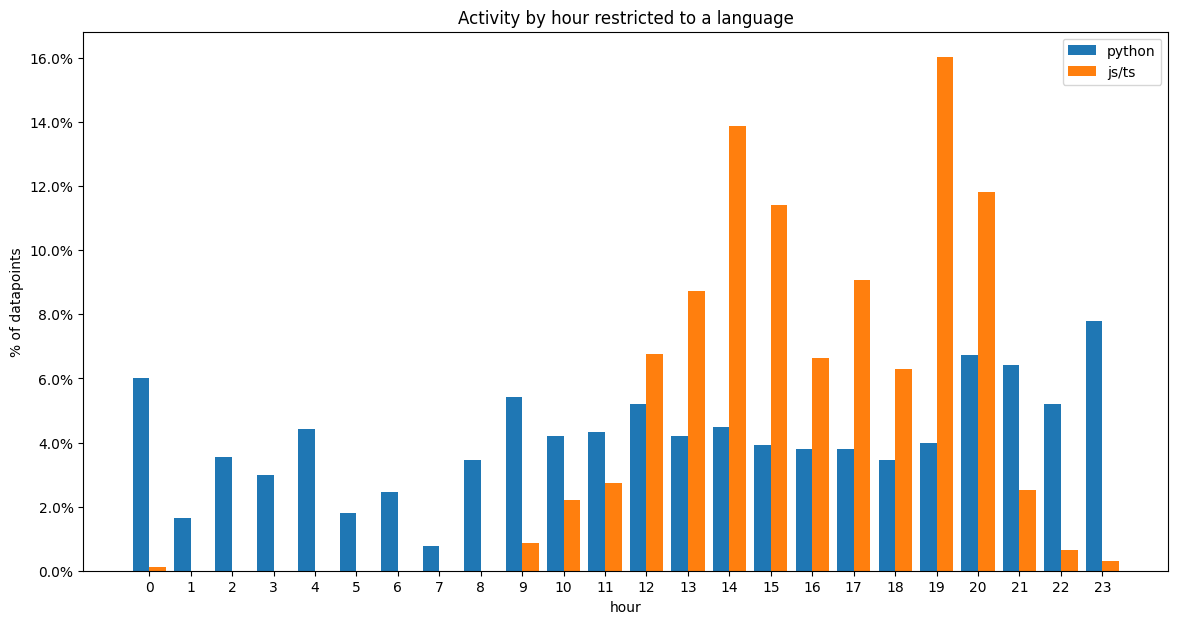
\includegraphics[scale=0.5]{chapters/results/graphics/activity-by-hour-langs.png}
  \caption{Comparison of activity by hour restricted to a language}
  \label{fig:activity_by_hour_langs}
\end{figure}

When it comes to performance measured as the average number of actions per data point, it remains relatively stable \ref{fig:performance_by_hour} with visible dips around the end of the standard working day (i.e. between 4 and 6 pm) and at night. Perceived anomalous surges during that period (i.e. at 12 and 5 am) occurred arguably due to smaller samples of data gathered at those time slots.

\begin{figure}[htbp]
  \centering
  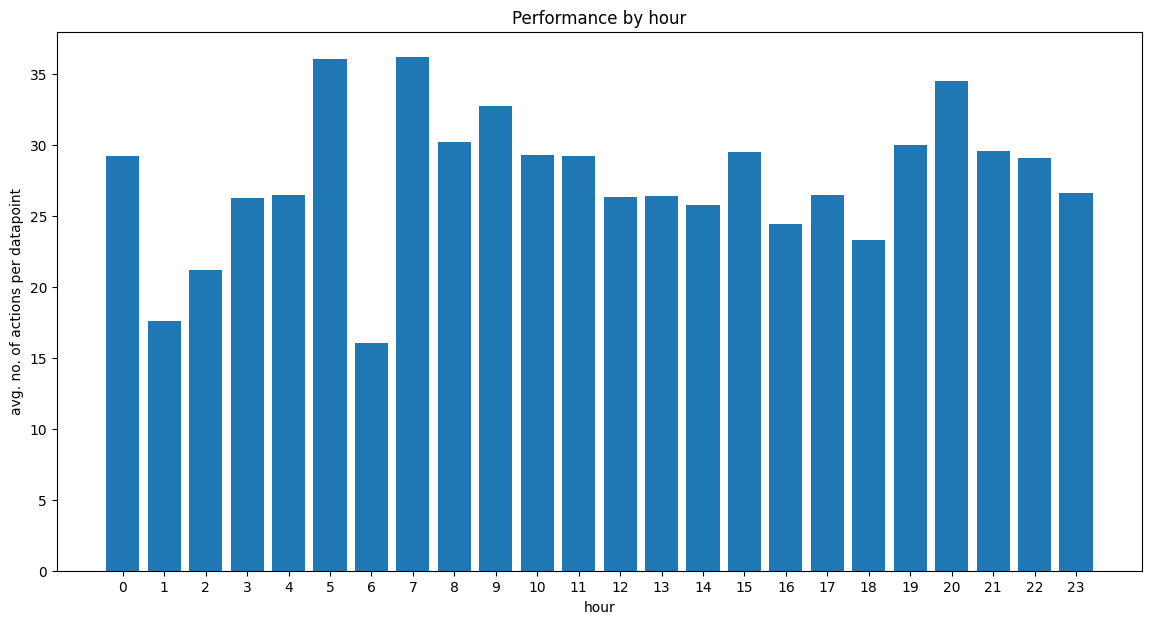
\includegraphics[scale=0.5]{chapters/results/graphics/performance-by-hour.png}
  \caption{Performance by hour}
  \label{fig:performance_by_hour}
\end{figure}

Such a trend is less clearly visible when restricted to Python and JS/TS languages \ref{fig:performance_by_hour_langs}, but this may be due to the fact that much less data was gathered at night and in the case of JS/TS even none in the majority of night hours. Comparing the results between the languages, it is noticeable that the performance metric for JS/TS developers is generally higher than for the Python ones (ignoring the night period).

\begin{figure}[htbp]
  \centering
  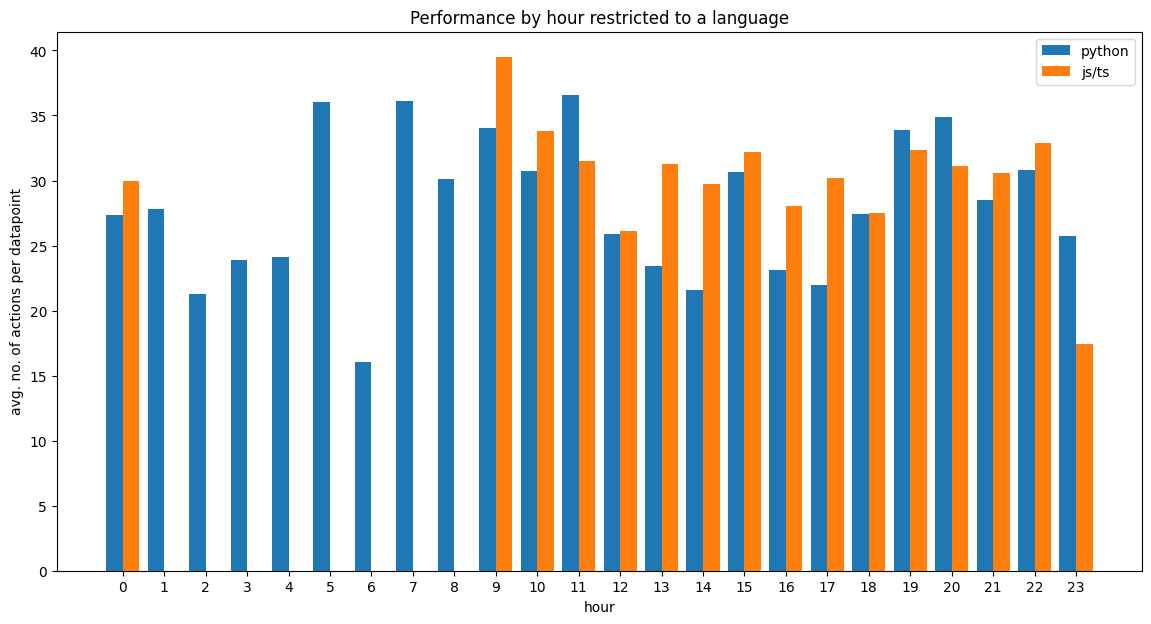
\includegraphics[scale=0.5]{chapters/results/graphics/performance-by-hour-langs.png}
  \caption{Performance by hour restricted to a language}
  \label{fig:performance_by_hour_langs}
\end{figure}
